% !TeX spellcheck = sk_SK-Slovak
% !TeX root = statnicaEKT.tex
\part{BPC-ESOT - Elektronické součástky}
%\chapter{ESOT}

\begin{huge}
	Otázky:
	\newline
\end{huge}
\begin{enumerate}
	\item Otázka - Bipolární tranzistor; struktura, princip činnosti. Nastavení a stabilizace pracovního bodu zesilovače ve třídě A. Zapojení SE, SB, SC. Bipolární tranzistor jako spínač, saturační zpoždění.
	\item Otázka - Unipolární tranzistory (JFET, MOSFET, MESFET); struktura a princip činnosti. Výstupní charakteristiky, převodní charakteristiky. FET jako proudový zdroj, zesilovač, spínač a řízený odpor.
	\item Otázka - Spínače. Tyristor; struktura, náhradní obvod, princip činnosti. Triak; struktura a princip činnosti. Tranzistor IGBT; struktura, náhradní obvod, princip činnosti. Řízení IGBT. Fázové řízení tyristorů. 
\end{enumerate}
\chapter{Bipolárny tranzistor}
\section{Štruktúra a princíp bipolárneho tranzistora}
\begin{itemize}
	\item Štruktúra bipolárneho tranzistora je založená na dvoch PN prechodoch $\rightarrow$ podľa typu tranzistora $\rightarrow$ PNP alebo NPN.
	\item Základom funkcie je odsávanie minoritných nosičov záverne polarizovaným prechodom.
	\begin{enumerate}
		\item \textbf{Odsávanie nosičov:} Na prechode kolektor-báza je napätie v závernom smere, čo spôsobuje efektívny zber (odsávanie) voľných nábojov do kolektora.
		\item \textbf{Injekcia z emitora:} Prechod báza-emitor je polarizovaný v priepustnom smere. To znižuje potenciálovú bariéru a umožňuje majoritným nosičom z emitora difúzne prechádzať do blízkej oblasti bázy.
		\item \textbf{Zmena na minority:} Nosiče, ktoré sa takto dostanú z emitora do bázy, sa v nej stávajú minoritnými nábojmi. Vďaka malej hrúbke bázy nezaniknú rekombináciou, ale driftujú k prechodu s kolektorom.
		\item \textbf{Riadený zdroj prúdu:} Kolektor odsaje takmer celý emitorový prúd. Tranzistor sa preto správa ako prúdový zdroj, kde je kolektorový prúd priamo riadený prúdom emitora.
		\item \textbf{Napäťové riadenie:} Výsledný prúd emitora (a tým aj celého tranzistora) nastavujeme veľkosťou priepustného napätia na prechode báza-emitor.
	\end{enumerate}
	\item Podmienky pre optimálnu činnosť PNP tranzistora:
	\begin{enumerate}
		\item Šírka báze musí byť menšia ako stredná difúzna dĺźka minoritných nosičov v báze. $\rightarrow$ \underline{báza musí byť veľmi tenká}
		\item Kontakt báze je vzdialený od emitorového prechodu niekoľko stredných difúznych dĺžkok
		\item Koncentrácia prímesí v emitore je omnoho väčšia ako koncentrácia prímesí v báze $\rightarrow$ \underline{emitor musí byť bohate dotovaný}
		\item Plocha kolektoru musí byť väčšia ako plocha emitora.
	\end{enumerate}
	\item Veľkosť kolektorového prúdu je daná veľkosťou napätia Báza - Emitor.
\end{itemize}
\begin{figure}[H]
	\centering
	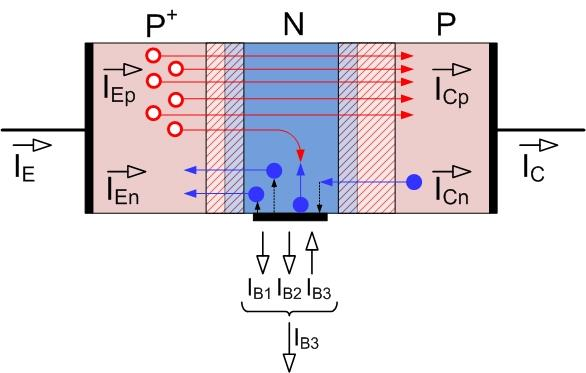
\includegraphics[width=0.5\linewidth]{Obrazky/ESOT/Otazka1/zlozkyPruduPNP}
	\caption{Zložky prúdu v tranzistore PNP}
	\label{fig:zlozkyprudupnp}
\end{figure}

\begin{figure}[H]
	\centering
	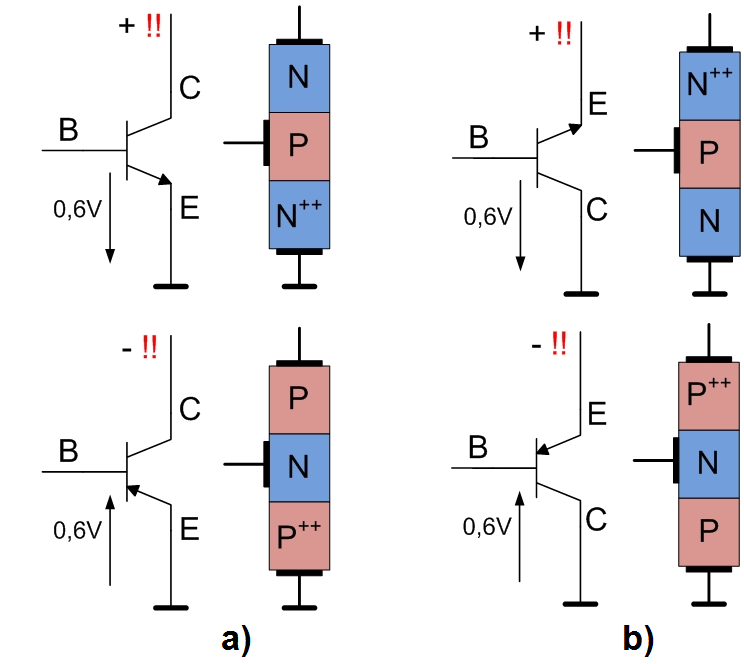
\includegraphics[width=0.5\linewidth]{Obrazky/ESOT/Otazka1/tranzistorStruktura}
	\caption{Idealizovaná štruktúra tranzistorov NPN a PNP, v normálnom a inverznom režime.}
	\label{fig:tranzistorstruktura}
\end{figure}
\section{Nastavenie pracovného bodu BJT zosilňovača a jeho stabilizácia v mostíkovom zapojení.}
BJT tranzistor pracuje pre zosilňovač ako zdroj prúdu, pričom výstupné napätie je tvorené rezistorom v kolektorovej ceste.
\begin{itemize}
	\item Nastavenie pracovného bodu znamená nastavenie prúdu bázou.
	\item Postup nastavenia pracovného bodu:
	\begin{itemize}
		\item Veľkosť bázového prúdu $I_B$ je nastavený bázovým rezistorom $R_B$
		\item V závislosti od nastavenia bázového prúdu $I_B$ je nastavný aj kolektorový prúd $I_C = \beta I_B$ 
		\item Úbytok napätia na $R_C$ je daný veľkosťou $I_C$, $U_RC = I_C R_C$
		\item Napätie na tranzistore je $U_{CE} = U_{CC} - U_{RC}$, kde $U_{CC}$ je napájacie napätie.
	\end{itemize}
	\item Pri nastavovaní pracovného bodu sa požaduje aby $U_{CE}$ bola polovica z napájacieho napätia, $U_{CE} = \frac{U_{CC}}{2}$
	\item V realite je však potrebné stabilizovať pracovný bod nakoľko je závislý od $\beta$ a teda je teplotne, tolerančne a rôzne inak závislý a nepresný.
\end{itemize}
\section{Stabilizácia pracovného bodu}
Používa sa zapojenie, kde pracovný bod tranzistora nie je závislý ani na prevádzkových podmienkach a ani na parametroch tranzistora.
\begin{itemize}
	\item \textbf{Stabilizácia pomocou zápornej spätnej väzby (odber prúdu z kolektoru):}
	\begin{itemize}
		\item \textbf{Princíp fungovania:} Prúd pre bázu sa odoberá z kolektora. Ak vzrastie kolektorový prúd ($I_C$), zvýši sa úbytok napätia na rezistore $R_C$. Tým klesne napätie dostupné pre rezistor $R_B$, zmenší sa bázový prúd $I_B$ a následne klesne aj $I_C$. Pri poklese prúdu to funguje opačne. Tento mechanizmus kompenzuje vplyv teploty, napájacieho napätia aj rozptyl parametrov tranzistora ($\beta$).
		\item \textbf{Postup návrhu / odhadu:} 
		\begin{itemize}
			\item Ak sa na kolektore nastaví polovica napájacieho napätia ($U_N / 2$), na odporoch $R_B$ a $R_C$ bude rovnaký úbytok napätia.
			\item Keďže odporom $R_B$ preteká $\beta$-krát menší prúd, musí byť jeho hodnota $\beta$-krát väčšia než $R_C$.
			\item Výsledný vzťah pre návrh: $R_B = \beta \cdot R_C$.
		\end{itemize}
	\end{itemize}
	
	\item \textbf{Môstková stabilizácia (pomocou prúdového zdroja s emitorovým odporom):}
	\begin{itemize}
		\item \textbf{Princíp fungovania:} Pracovný bod sa stabilizuje pomocou emitorového rezistora $R_E$. Aby tento rezistor neovplyvňoval striedavý signál (neznižoval zosilnenie), premosťuje sa blokovacím kapacitorom $C_E$. Odporový delič v báze ($R_{B1}, R_{B2}$) musí byť dostatočne „tvrdý“ vzhľadom na vstupný odpor tranzistora ($\beta \cdot R_E$), aby prúd bázy podstatne nemenil napätie na báze $U_B$.
		\item \textbf{Postup návrhu:}
		\begin{enumerate}
			\item Rozdelí sa napájacie napätie rovnomerne medzi súčiastky: $U_{RC} \approx U_{CE} \approx U_{RE} \approx \frac{U_N}{3}$.
			\item Zvolí sa emitorový prúd $I_E$ a vypočíta sa emitorový odpor: $R_E = \frac{U_{RE}}{I_E} = \frac{U_N}{3 I_E}$.
			\item Keďže platí $I_E \approx I_C$ a $U_{RC} \approx U_{RE}$, zvolí sa kolektorový odpor: $R_C \approx R_E$.
			\item Navrhne sa napäťový delič v báze tak, aby bol dostatočne tvrdý: zvolí sa $R_{B2} < \beta \cdot R_E$ a následne druhá vetva $R_{B1} \approx 2 \cdot R_{B2}$.
			\item Navrhne sa kapacita $C_E$ tak, aby jej impedancia bola na najnižšom pracovnom kmitočte rádovo menšia ako veľkosť odporu $R_E$.
		\end{enumerate}
	\end{itemize}
\end{itemize}

\begin{figure}[H]
	\begin{subfigure}[b]{0.48\textwidth}
		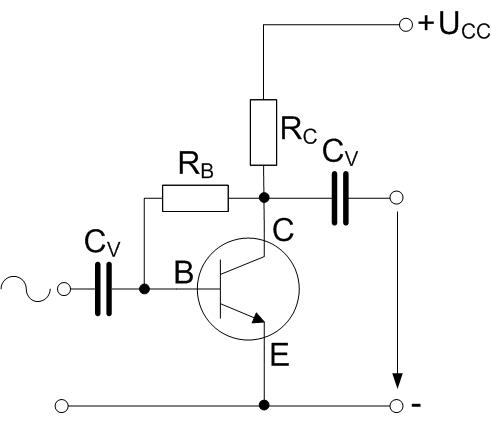
\includegraphics[width=0.7\linewidth]{Obrazky/ESOT/Otazka1/stabilizaciaKZV}
		\caption{Stabilizácia pracovného bodu s pomocou zápornej spätnej väzby.}
		\label{fig:stabilizaciakzv}
	\end{subfigure}
	\begin{subfigure}[b]{0.48\textwidth}
		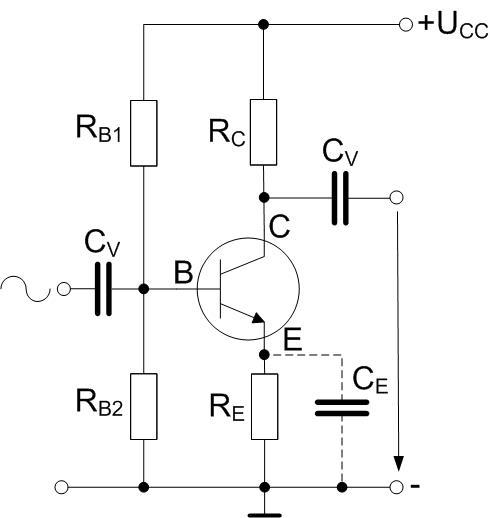
\includegraphics[width=0.7\linewidth]{Obrazky/ESOT/Otazka1/stabilizaciaMostik}
		\caption{Stabilizácia s pomocou emitorového odporu (Štandardne používané).}
		\label{fig:stabilizaciamostik}
	\end{subfigure}	
\end{figure}
\section{Základné zapojenia bipolárneho tranzistora}
\begin{figure}[H]
	\centering
	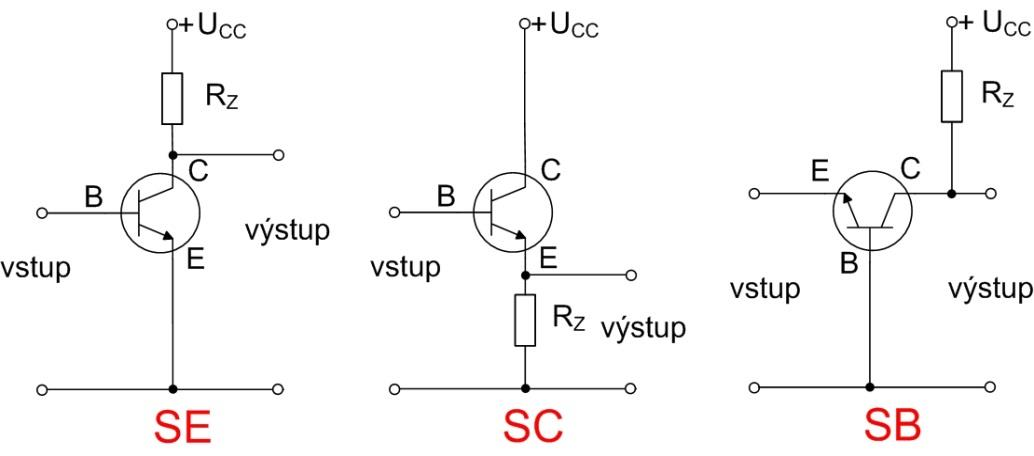
\includegraphics[width=0.7\linewidth]{Obrazky/ESOT/Otazka1/zakladneZapojeniaTranzistora}
	\caption{Základné zapojenia bipolárneho tranzistora.}
	\label{fig:zakladnezapojeniatranzistora}
\end{figure}

\begin{itemize}
	\item \textbf{Zapojenie so spoločným emitorom (SE):}
	\begin{itemize}
		\item \textbf{Vlastnosti:} Najpoužívanejšie zapojenie s najväčším \textbf{výkonovým zosilnením} (dané súčinom veľkého napäťového a veľkého prúdového zosilnenia $\beta$).
		\item \textbf{Fáza:} Otáča fázu striedavého signálu o $180^\circ$ (výstup je v protifázi voči vstupu).
		\item \textbf{Impedancie:} Malý vstupný odpor (priepustne polarizovaný prechod B-E) a veľký výstupný odpor (záverne polarizovaný prechod C-B).
	\end{itemize}
	
	\item \textbf{Zapojenie so spoločným kolektorom (SC / Emitorový sledovač):}
	\begin{itemize}
		\item \textbf{Vlastnosti:} Napäťové zosilnenie je približne rovné $1$ (výstupné napätie na emitore sleduje vstup na báze), prúdové zosilnenie je veľké ($\beta$).
		\item \textbf{Fáza:} Neotáča fázu (vstup a výstup sú vo fáze).
		\item \textbf{Impedancie:} \textbf{Veľký vstupný odpor} (daný súčinom odporu v emitore $R_Z$ a činiteľa $\beta$) a \textbf{veľmi malý výstupný odpor}. Používa sa najmä ako impedančné prispôsobenie (oddeľovací stupeň).
	\end{itemize}
	
	\item \textbf{Zapojenie so spoločnou bázou (SB):}
	\begin{itemize}
		\item \textbf{Vlastnosti:} Veľké napäťové zosilnenie (porovnateľné so SE), ale prúdové zosilnenie ($\alpha$) je \textbf{menšie ako 1}. Výkonové zosilnenie je preto relatívne malé. Výhodou je vysoký medzný kmitočet ($f_\alpha \gg f_\beta$).
		\item \textbf{Fáza:} Neotáča fázu (vstup a výstup sú vo fáze).
		\item \textbf{Impedancie:} \textbf{Veľmi malý vstupný odpor} (prechod E-B v priepustnom smere) a veľký výstupný odpor.
		\item \textbf{Použitie:} Dnes už výnimočné (vysokofrekvenčné obvody, kaskódy, diferenciálne zosilňovače). Z princípu tohto zapojenia vznikol názov tranzistor (\textit{TRANSfer resISTOR} – prenos prúdu z nízkej impedancie na vysokú).
	\end{itemize}
\end{itemize}
\section{Tranzistor ako spínač}
\begin{itemize}
	\item \textbf{Pracovné stavy spínača:}
	\begin{itemize}
		\item \textbf{Stav SEPNUTO (Vodivý):} Do bázy sa vnúti veľký prúd. Tranzistor prejde do \textbf{saturácie (nasýtenia)}, kedy je prechod B-C polarizovaný v priepustnom smere. Napätie $U_{CE}$ klesne na minimum ($U_{CES} \approx$ desiatky mV až 1 V). Vodivostné straty sú dané vzťahom $P_Z = I_C \cdot U_{CES}$. Náhradný odpor v zopnutom stave je minimálny ($R_{ON} \approx$ jednotky $\Omega$).
		\item \textbf{Stav ROZEPNUTO (Nevodivý):} Obvodom preteká len minimálny zbytkový prúd. Na jeho potlačenie sa báza spája s emitorom cez malý odpor ($R_{BE} < 100\,\Omega$), ktorý odvedie časť nežiaduceho náboja. Náhradný odpor je obrovský ($R_{OFF} \approx \text{k}\Omega \text{ až M}\Omega$).
	\end{itemize}
	
	\item \textbf{Saturačné oneskorenie ($t_s$):}
	\begin{itemize}
		\item \textbf{Problém:} V saturácii sa kvôli zlej odsávacej schopnosti kolektora hromadia v báze nadbytočné minoritné nosiče. Pri vypínaní tranzistora vzniká časové zpoždenie ($t_s$), pretože tieto nosiče musia najprv zrekombinovať alebo sa odvést, až potom sa tranzistor reálne uzavrie. Celkový čas vypnutia je $t_{OFF} = t_s + t_f$.
		</itemize>
		
		\item \textbf{Postupy na zrýchlenie spínania (skrátenie $t_s$):}
		\begin{enumerate}
			\item \textbf{Rekombinačné centrá:} Technologické zavedenie prímesí do bázy urýchľuje zánik náboja, nevýhodou je ale trvalé zníženie zosilňovacieho činiteľa $\beta$ (v aktivnom režime max. 50).
			\item \textbf{Urýchľovací kapacitor:} Zapojenie kondenzátora $C_B$ paralelne k bázovému odporu $R_B$. Pri zostupnej hrane pomáha rýchlo odsať náboj z bázy.
			\item \textbf{Nenasýtený režim:} Obvodové zaistenie, aby tranzistor nikdy neprešiel do hlbokej saturácie a zostal v aktívnom režime (napr. ECL logika).
			\item \textbf{Schottkyho desaturačná dióda:} Zapája sa medzi bázu a kolektor. Odoberá prebytočný bázový prúd a zabraňuje hlbokej saturácii. \textbf{Nevýhoda:} Zvyšuje napätie $U_{CE}$ v zopnutom stave, čo výrazne zvyšuje trvalé vodivostné straty $P_Z$.
		\end{enumerate}
	\end{itemize}
	\item \textbf{Spínač v inverznom zapojení (obrátená funkcia emitora a kolektora):}
	\begin{itemize}
		\item \textbf{Princíp fungovania:} Výmena úloh prechodov – emitorový prechod náboj odsáva a kolektorový ho injektuje. Tranzistorový jav ostáva zachovaný, ale funguje s odlišnými parametrami kvôli nesymetrii dotovania a plôch prechodov.
		\item \textbf{Nevýhody:}
		\begin{itemize}
			\item \textbf{Prudký pokles zosilnenia:} Kvôli nízkej koncentrácii prímesí v kolektore a malej ploche emitora klesá prúdový zosilňovací činiteľ ($\beta_{inv}$) takmer o dva rady (typicky má hodnotu \textbf{menšiu ako 10}).
			\item \text{\textbf{Malé záverné napätie:}} Odsávajúci prechod emitor-báza znesie kvôli vysokej koncentrácii prímesí v emitore napätie len v rozsahu \textbf{6 V až 7 V}.
		\end{itemize}
		\item \textbf{Hlavná výhoda:} Umožňuje dosiahnuť \textbf{extrémne malé saturačné napätie} $U_{ECS}$ (typicky len \textbf{niekoľko mV}, zatiaľ čo v normálnom režime sú to desiatky mV). Zapojenie je preto ideálne pre spínanie signálov s veľmi nízkou úrovňou napätia a prúdov.
		\item \textbf{Príčina nízkeho saturačného napätia:} 
		\begin{enumerate}
			\item Silne dotovaný prechod báza-emitor má väčšie difúzne napätie, čo mu dáva lepšiu odsávaciu schopnosť pri prepolarizovaní v saturácii.
			\item Na prechode báza-kolektor je menší úbytok napätia v priepustnom smere, takže tranzistor prechádza do saturácie pri omnoho menšom napätí $U_{EC}$.
		\end{enumerate}
	\end{itemize}
\end{itemize}
\begin{figure}[H]
	\begin{subfigure}[b]{0.48\textwidth}
		\centering
		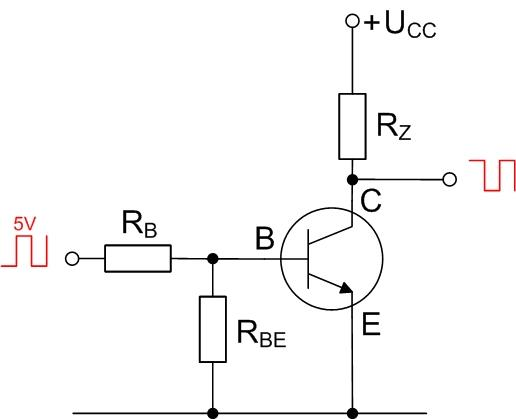
\includegraphics[width=0.7\linewidth]{Obrazky/ESOT/Otazka1/tranzistorovySpinac}
		\caption{Tranzistor ako spínač - NPN tranzistor.}
		\label{fig:tranzistorovyspinac}
	\end{subfigure}
	\begin{subfigure}[b]{0.48\textwidth}
		\centering
		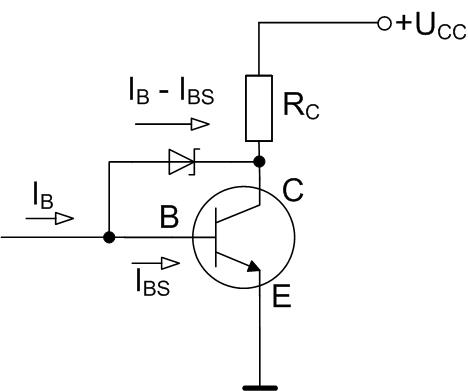
\includegraphics[width=0.7\linewidth]{Obrazky/ESOT/Otazka1/saturacnaDioda}
		\caption{Spínač so Schottkyho desaturačnou diódou.}
		\label{fig:saturacnadioda}
	\end{subfigure}	
\end{figure}
\begin{figure}[H]
	\centering
	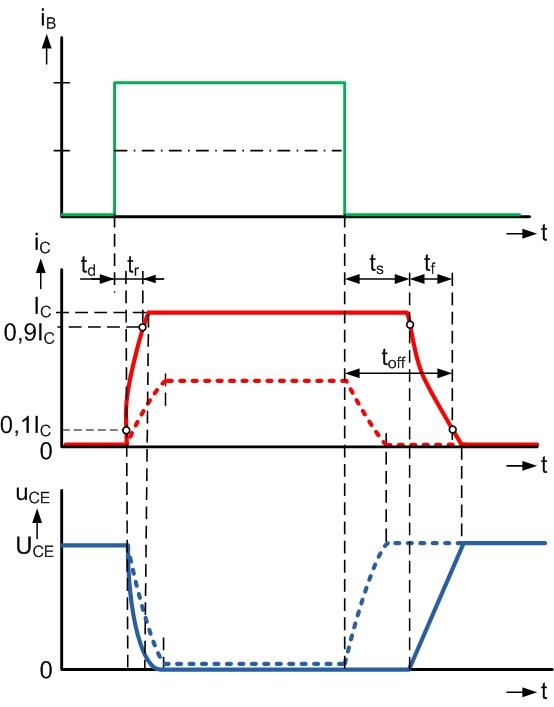
\includegraphics[width=0.5\linewidth]{Obrazky/ESOT/Otazka1/priebehySpinania}
	\caption{Priebeh rozopnutia tranzistora v nasýtenom a nenasýtenom stave.}
	\label{fig:priebehyspinania}
\end{figure}

\chapter{Unipolárne tranzistory}

V unipolárnych tranzistoroch sa vedenie prúdu uskutočňuje iba jedným typom nosičov - majoritné. Koncentrácia týchto nosičov a ich pohyb pritom závisia od veľkosti a polarity elektrického poľa medzi riadiacou elektródou a vodivým kanálom tranzistora. Elektrické pole pod riadiacou elektródou G vyvoláva zmenu prierezu vodivého kanála.

V súčasnosti delíme unipolárne tranzistory na tri základné typy:
\begin{enumerate}
	\item \textbf{Tranzistory s prechodovým hradlom (JFET} [Junction-FET]) – princíp funkcie spočíva v zmene prierezu vodivého kanála rozširovaním depletovanej (závernej) vrstvy prechodu polarizovaného v závernom smere.
	\item \textbf{Tranzistory s izolovaným hradlom (IGFET} [Insulated Gate FET] / \textbf{MOSFET}) – princíp funkcie spočíva v zmene koncentrácie minoritných nosičov pritiahnutých zo substrátu v takom množstve, že vytvoria kanál s inverzným typom vodivosti, než je vodivosť substrátu.
	\item \textbf{Tenkovrstvové tranzistory s izolovaným hradlom (TFT} [Thin Film Transistors]) – pracujú na podobnom princípe ako tranzistory IGFET. Ich zvláštnosťou je odlišné riadenie a funkcia elektród. Tenkovrstvové technológie umožňujú použitie tranzistorov TFT v displejoch a ďalších veľkoplošných aplikáciách.
	\item Ďalej sa delia podľa typu kanálu $\rightarrow$ P alebo N.
\end{enumerate}

Pracujú iba s majoritnými nosičmi, ich zapínacie a vypínacie časy sú dané hlavne parazitnými kapacitami, ktoré sa musia nabiť a vybiť pri každom zopnutí a vypnutí, nie sú teplotne závislé, a preto časy $t_{\text{on}}$ a $t_{\text{off}}$ nezávisia od teploty. Nie je tu jav akumulácie minoritných nosičov. 

\section{JFET – Unipolárny tranzistor s prechodom PN}

\section{Štruktúra a princíp činnosti}
Vlastná pracovná oblasť tranzistora JFET sa nazýva kanál (napr. s vodivosťou typu N). Kanál ústi do dvoch oblastí, ktoré sú opatrené neusmerňujúcimi kontaktmi:
\begin{itemize}
	\item \textbf{S (Source)} – zdroj, obdoba emitora.
	\item \textbf{D (Drain)} – odtok, nora, zberná elektróda, obdoba kolektora.
	\item \textbf{G (Gate)} – hradlo, je pripojené na oblasť s opačným typom vodivosti než kanál (pri N-kanáli je to oblasť $\text{P}^+$).
\end{itemize}

Pri riadení vodivosti kanála je prechod $\text{P}^+\text{N}$ medzi hradlom a kanálom polarizovaný v závernom smere. Prechod sa preto v závislosti od napätia $U_{\text{GS}}$ rozširuje (depletovaná oblasť sa rozširuje do menej dotovanej oblasti N). Zmenou šírky prechodu sa mení prierez kanála, jeho vodivosť a tým aj prúd $I_{\text{D}}$ pretekajúci medzi elektródami S a D.

Činnosť štruktúry JFET v závislosti od pripojeného napätia:
\begin{itemize}
	\item \textbf{Pri $U_{\text{GS}} = 0\,\text{V}$:} Prechod $\text{P}^+\text{N}$ je v termodynamickej rovnováhe, šírka prechodu je minimálna a prierez kanála maximálny. Ak sa zvýši napätie $U_{\text{DS}}$ nad nulu, prúd $I_{\text{D}}$ vzrastá spočiatku lineárne. Tranzistor sa chová ako lineárny rezistor riadený napätím $U_{\text{GS}}$.
	\item \textbf{Vplyv $U_{\text{DS}}$ a zaškrtenie kanála:} Pretože sa kanál chová ako odporový prvok, dôjde po priložení napätia $U_{\text{DS}}$ k rozdeleniu potenciálu pozdĺž kanála. Zo strany elektródy D je potenciál kanála proti hradlu najkladnejší, prechod je tu najviac polarizovaný v závernom smere a najviac sa rozširuje. Prierez kanála sa na strane elektródy D zmenšuje, odpor kanála rastie a prúd rastie pomalšie.
	\item \textbf{Saturácia:} Pri dosiahnutí saturačného napätia $U_{\text{DS}} = U_{\text{DSsat}}$ dôjde k úplnému zaškrteniu vodivého kanála na strane elektródy D. Pre napätia $U_{\text{DS}} \ge U_{\text{DSsat}}$ sa veľkosť prúdu kanálom už takmer nemení a dosahuje hodnotu saturačného prúdu $I_{\text{Dsat}}$. Priložené napätie prevyšujúce $U_{\text{DSsat}}$ sa prejaví predovšetkým ako úbytok napätia na zaškrtenej časti kanála $\Delta L$. Nosiče sú cez zaškrtenú oblasť odsávané elektrickým polom.
	\item \textbf{Prieraz:} Pri zvýšení napätia $U_{\text{DS}}$ nad hodnotu $U_{\text{DSmax}}$ dôjde k lavínovému prierazu zaškrtenej časti kanála (tepelný prieraz a zničenie súčiastky).
\end{itemize}
\begin{figure}[H]
	\centering
	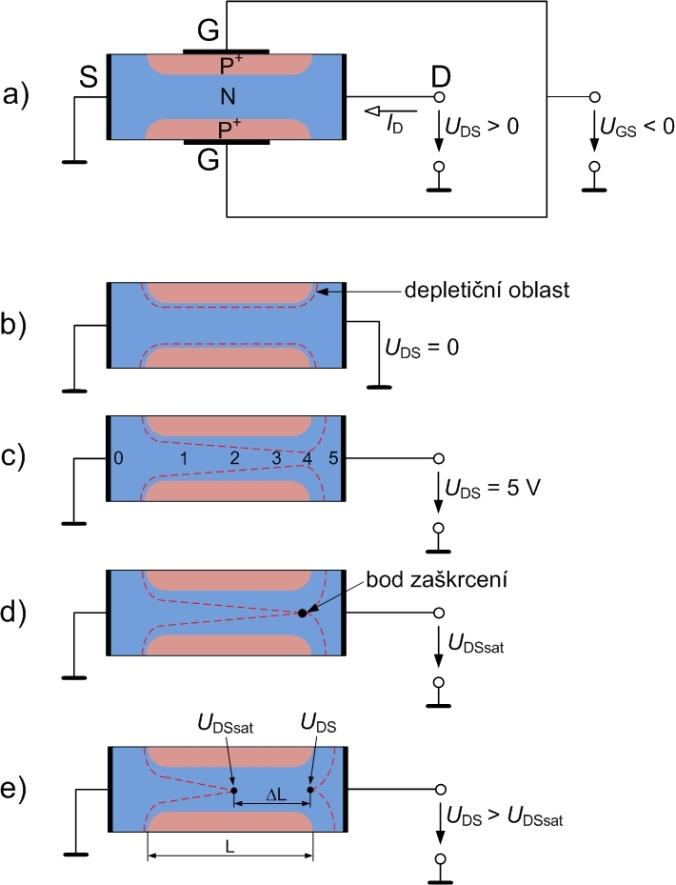
\includegraphics[width=0.4\linewidth]{Obrazky/ESOT/Otazka2/jfetModyStruktura}
	\caption{Znázornenie jednotlivých fází činností tranzistoru JFET.}
	\label{fig:jfetmodystruktura}
\end{figure}
\begin{figure}[H]
	\centering
	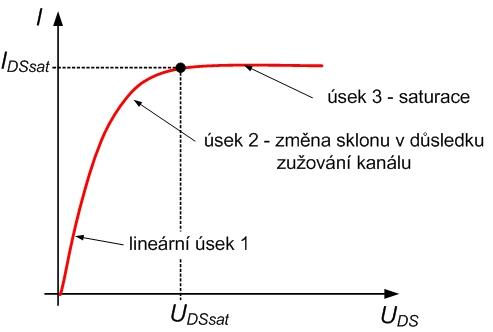
\includegraphics[width=0.5\linewidth]{Obrazky/ESOT/Otazka2/vystupnaCharJFET}
	\caption{Výstupná ampérvoltová charakterisitka JFET.}
	\label{fig:vystupnacharjfet}
\end{figure}
\begin{figure}[H]
	\centering
	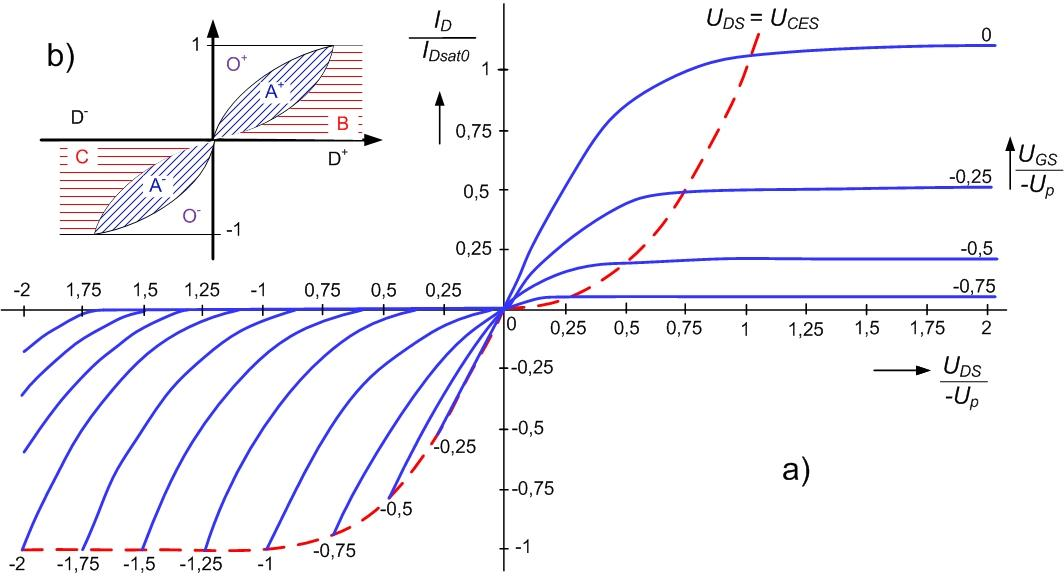
\includegraphics[width=0.7\linewidth]{Obrazky/ESOT/Otazka2/normovaneVystupneApracovne}
	\caption{Normované výstupné charakteristiky (a) a pracovné oblasti tranzistoru P-JFET (b).}
	\label{fig:normovanevystupneapracovne}
\end{figure}
\begin{itemize}
	\item Aktívny režim $\rightarrow$ písmeno A $\rightarrow$ základný pracovný režim JFET $\rightarrow$ lineárna časť char.
	\item Saturačný režim $\rightarrow$ písmeno B
	\item Triódový režim $\rightarrow$ písmeno C
	\item Uzavretý režim $\rightarrow$ písmeno D
\end{itemize}
\begin{figure}[H]
	\centering
	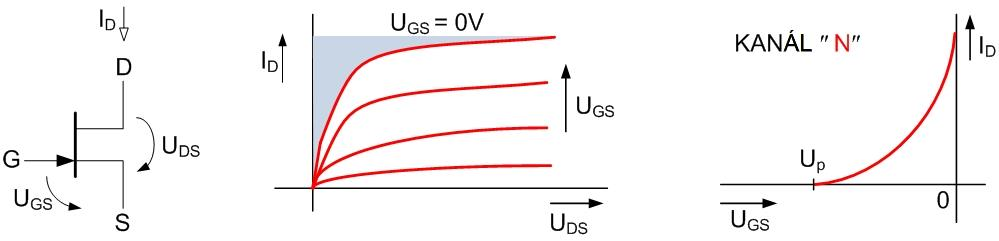
\includegraphics[width=0.7\linewidth]{Obrazky/ESOT/Otazka2/prenosoveaVystupneCharJFET1}
	\caption{Prevodová a výstupná charakteristika N-JFET.}
	\label{fig:prenosoveavystupnecharjfet1}
\end{figure}

\begin{figure}[H]
	\centering
	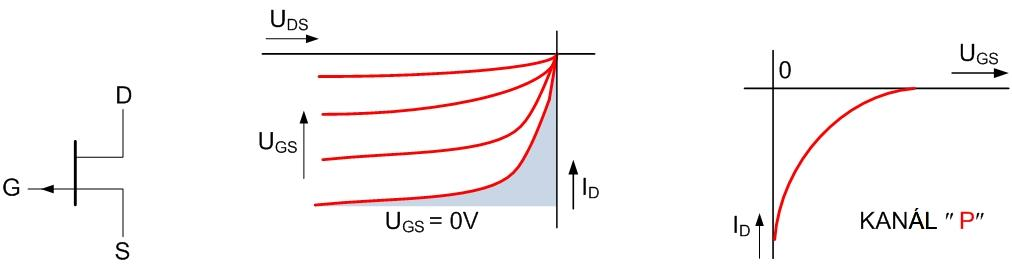
\includegraphics[width=0.7\linewidth]{Obrazky/ESOT/Otazka2/prenosoveaVystupneCharJFET}
	\caption{Prevodová a výstupná charakteristika P-JFET.}
	\label{fig:prenosoveavystupnecharjfet}
\end{figure}

%\section{Riadenie vodivosti kanála a prahové napätie}
%Pre $U_{\text{GS}} < 0\,\text{V}$ (pre N-kanál) je prechod polarizovaný v závere, depletovaná vrstva je širšia a kanál užší:
%1. Počiatočná vodivosť kanála je menšia, prúd $I_{\text{D}}$ vzrastá pomalšie.
%2. K zaškrteniu kanála dochádza skôr, hodnoty $U_{\text{DSsat}}$ a $I_{\text{Dsat}}$ sú menšie.
%3. Pri dostatočne veľkom závernom napätí sa depletovaná vrstva rozšíri cez celú šírku kanála a prúd klesne na nulu. Toto napätie sa nazýva \textbf{prahové napätie} $U_{\text{P}}$ (v anglickej literatúre $U_{\text{T}}$ alebo $V_{\text{T}}$ [Threshold voltage]).

%\section{Pracovné režimy a charakteristiky JFET}
%Chovanie tranzistora je popísané sieťou výstupných ($I_{\text{D}} = f(U_{\text{DS}})$ pri $U_{\text{GS}} = \text{const.}$) a prevodných charakteristík ($I_{\text{D}} = f(U_{\text{GS}})$ pri $U_{\text{DS}} = \text{const.}$).
%
%Tranzistor JFET môže pracovať v týchto režimoch:
%\begin{enumerate}
%	\item \textbf{Aktívny režim (A):} Základný režim. Delí sa na $A^+$ (pri kladnom $U_{\text{DS}}$ v I. kvadrante) a $A^-$ (pri zápornom $U_{\text{DS}}$ v III. kvadrante). Režim $A^+$ prechádza pri zvýšení $U_{\text{DS}}$ do saturačného režimu B. Hranica je určená podmienkou:
%	\begin{equation}
%		U_{\text{DS}} = U_{\text{DSsat}} = U_{\text{GS}} - U_{\text{P}}
%	\end{equation}
%	\item \textbf{Saturačný režim (B):} Veľkosť prúdu $I_{\text{D}}$ nezávisí od $U_{\text{DS}}$. Závislost prúdu od riadiaceho napätia je kvadratická a dá sa popsať vzťahom:
%	\begin{equation}
%		I_{\text{D}} = f(U_{\text{GS}} - U_{\text{P}})^2 \implies I_{\text{D}} = \frac{I_{\text{DSS}}}{U_{\text{P}}^2} (U_{\text{P}} - U_{\text{GS}})^2
%	\end{equation}
%	Kde $I_{\text{DSS}}$ je saturačný prúd pri $U_{\text{GS}} = 0\,\text{V}$. S uzatváraním kanála (rastúca absolútna hodnota $U_{\text{GS}}$) sa vzdialenosť medzi charakteristikami zmenšuje.
%	\item \textbf{Nulový režim ($0^+ / 0^-$):} Nastáva pri prekročení $U_{\text{GS}} = 0\,\text{V}$ do kladných hodnôt (prakticky od $+0,5\,\text{V}$), kedy prechod hradlo-kanál prejde do propustného smeru, hradlom tečie prúd a tranzistor nepracuje správne.
%	\item \textbf{Triódový režim (C):} Tranzistor doňho prechádza pre hodnoty $U_{\text{GS}} < U_{\text{P}}$ a $U_{\text{DS}} < 0\,\text{V}$. Každá z charakteristík končí pri hodnote $U_{\text{DS}} = U_{\text{GS}} < 0\,\text{V}$, kde prechádza do režimu $0^-$. Využíva sa v režime uzavretého spínača (napr. spínanie striedavého napätia). Pre spoľahlivé uzavretie spínača s amplitúdou signálu $U_{\text{M}}$ musí platiť:
%	\begin{equation}
%		|U_{\text{GS}}| > (|U_{\text{P}}| + |U_{\text{M}}|)
%	\end{equation}
%	\item \textbf{Režim D (Stav uzavretia):} Celý kanál je uzavretý a tranzistorom netečie žiadny prúd.
%\end{enumerate}
%
%\section{Typy tranzistorov JFET}
%\begin{itemize}
%	\item \textbf{N-JFET:} Kanál typu N, hradlo P. Riadi sa záporným napätím $U_{\text{GS}}$, pričom $U_{\text{DS}}$ a $I_{\text{D}}$ sú kladné.
%	\item \textbf{P-JFET:} Vyrobený na substráte typu P. Polarity všetkých prúdov a napätí sú opačné ($U_{\text{DS}}$ a $I_{\text{D}}$ sú záporné, $U_{\text{GS}}$ je kladné). Šípka v schematickej značke smeruje od tranzistora von.
%\end{itemize}
%
%\section{Nastavenie pracovného bodu a zosilňovač s JFET}
%Strmosť prevodnej charakteristiky $g_{\text{m}}$ získame deriváciou aproximačnej rovnice v danom pracovnom bode:
%\begin{equation}
%	g_{\text{m}} = \frac{dI_{\text{D}}}{dU_{\text{GS}}} = -2 \left( \frac{I_{\text{DSS}}}{U_{\text{P}}^2} \right) (U_{\text{P}} - U_{\text{GS}})
%\end{equation}
%Pre napäťové zosilnenie zapojenia so spoločným zdrojom (SS) platí:
%\begin{equation}
%	A_{\text{U}} = -|g_{\text{m}}| R_{\text{D}}
%\end{equation}
%Pre udržanie tranzistora v saturácii musí platiť podmienka pre zaťažovací odpor $R_{\text{D}}$:
%\begin{equation}
%	R_{\text{D}} < \frac{U_{\text{DD}} - U_{\text{GS}} + U_{\text{P}}}{I_{\text{D}}}
%\end{equation}
%
%Metódy nastavenia pracovného bodu $P [I_{\text{DP}}, U_{\text{GSP}}]$:
%\begin{itemize}
%	\item \textbf{Externým zdrojom v hradle:} Vyžaduje ďalší záporný napájací zdroj.
%	\item \textbf{Automatické predpätie pomocou rezistora $R_{\text{S}}$:} Využíva úbytok napätia na rezistore v emitorovej (zdrojovej) elektróde. Hradlo je uzemnené cez veľký odpor $R_{\text{G}}$ (cca $1\,\text{M}\Omega$). Hodnota rezistora sa určí ako:
%	\begin{equation}
%		R_{\text{S}} = \frac{U_{\text{GS}}}{I_{\text{D}}}
%	\end{equation}
%	Nevýhodou je zmenšenie využiteľného napäťového rozsahu a vznik zápornej striedavej spätnej väzby (potláča sa paralelným kapacitorom $C_{\text{S}}$).
%	\item \textbf{Mostíkové zapojenie s deličom napätia ($R_1, R_2$) a $R_{\text{S}}$:} Stabilizuje pracovný bod pri technologickom rozptyle prahového napätia tranzistorov. Veľkosť rezistora $R_{\text{S}}$ se určí podľa vzťahu:
%	\begin{equation}
%		R_{\text{S}} = \frac{U_{\text{G}} + U_{\text{GSS}}}{I_{\text{D}}}
%	\end{equation}
%	Kde $U_{\text{G}}$ je napätie na hradle z deliča a $U_{\text{GSS}}$ je stredná predpokladaná hodnota $U_{\text{GS}}$.
%\end{itemize}
%
%\section{Teplotné a kmitočtové závislosti JFET}
%\begin{itemize}
%	\item \textbf{Kmitočtová závislosť:} Pri DC aplikáciách je vstupný odpor daný záverným prúdom prechodu (cca $10^9\,\Omega$). Pri zvyšovaní kmitočtu sa uplatňujú parazitné kapacity a okolo $100\,\text{kHz}$ klesá vstupná impedancia na rád $10^4\,\Omega$.
%	\item \textbf{Teplotná závislosť:} Mnohom menšia ako pri bipolárnych tranzistoroch. V oblasti malých prúdov $I_{\text{D}}$ prúd s teplotou rastie, v oblasti veľkých prúdov s teplotou klesá. Existuje bod (kríženie charakteristík), kde prúd nezávisí od teploty. Pokles prúdu s teplotou pri vyššom zaťažení umožňuje paralelné radenie tranzistorov (nehrozí tepelné utrhnutie). Strmosť $g_{\text{m}}$ a zosilnenie s rastúcou teplotou mierne klesajú.
%\end{itemize}
%
\section{IGFET / MOSFET – Unipolárny tranzistor s izolovanou riadiacou elektródou}

\section{Štruktúra a princíp činnosti}
Pri tranzistoroch typu \textbf{IGFET} (Insulated Gate FET) alebo \textbf{MOSFET} (Metal Oxide Semiconductor FET) ovláda elektrické pole cez tenkú vrstvu izolantu (pôvodne výhradne $\text{SiO}_2$) vytváranie vodivého kanála, ktorý má opačný (inverzný) typ vodivosti než substrát, na ktorom je štruktúra vytvorená.

Štruktúra pozostáva z:
\begin{itemize}
	\item \textbf{Substrátu} (napr. typ P).
	\item \textbf{Oblastí S a D} s opačným typem vodivosti než substrát (napr. $\text{N}^+$). Medzi S a D sú teda dva prechody PN zapojené proti sebe – bez vonkajšieho poľa prúd nepreteká.
	\item \textbf{Hradla G}, ktoré je od substrátu oddelené tenkou vrstvou izolantu.
\end{itemize}

\textbf{Mechanizmus vzniku kanála (pre indukovaný N-kanál na substráte P):}
\begin{enumerate}
	\item Priložením kladného napätia $U_{\text{GS}}$ sa najprv odpudia majoritné nosiče (diery) od povrchu substrátu pod hradlom. Zostane tu náboj ionizovaných prímesí, ale prúd stále nepreteká.
	\item  Pri ďalšom zvýšení napätia nad \textbf{prahové napätie} $U_{\text{P}}$ sú k povrchu pritiahnuté minoritné nosiče (elektróny) zo substrátu. Vytvorí sa tenká \textbf{inverzná vrstva} (kanál typu N), ktorá vodivo prepojí oblasti S a D. Vodivosť kanála rastie približne kvadraticky s $U_{\text{GS}}$.
	\item  Pri malom napätí $U_{\text{DS}}$ sa kanál chová ako lineárny rezistor.
	\item  Pri zvyšovaní $U_{\text{DS}}$ sa potenciál medzi kanálom a hradlom na strane elektródy D zmenšuje, koncentrácia nosičov tu klesá a kanál sa zaškrcuje. Pri dosiahnutí saturácie sa tranzistor chová ako prúdový zdroj (rovnako ako JFET).
	\item  Pri zápornom $U_{\text{DS}}$ (režim spínača) dochádza k otváraniu kanála. Pre spoľahlivé uzavretie striedavého signálu je nutné na hradlo priviesť dostatočne veľké záporné napätie, limitované maximálnym povoleným napätím hradla ($20$ až $25\,\text{V}$).
\end{enumerate}

\begin{figure}[H]
	\centering
	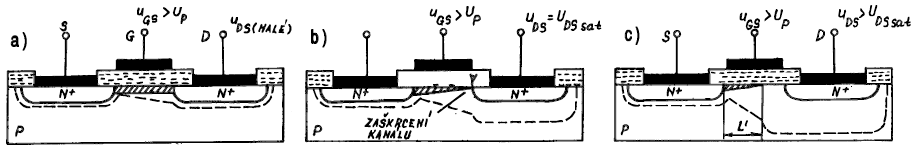
\includegraphics[width=\linewidth]{Obrazky/ESOT/Otazka2/strukturaIGFET}
	\caption{Tranzistor IGFET s indukovaným kanálom typu N.}
	\label{fig:strukturaigfet}
\end{figure}

\section{Typy tranzistorov IGFET / MOSFET}
Tranzistory IGFET existujú v štyroch základných variantoch podľa typu vodivosti kanála a technologického prevedenia:

\begin{enumerate}
	\item \textbf{Tranzistor s indukovaným kanálom (obohacovací modifikácia, enhancement):} Kanál vzniká až po priložení dostatočného napätia $U_{\text{GS}} > U_{\text{P}}$. Pri $U_{\text{GS}} = 0\,\text{V}$ je tranzistor úplne uzavretý ($I_{\text{D}} = 0$).
	\item \textbf{Tranzistor s trvalým kanálom (ochudobňovacia modifikácia, depletion):} Vodivý kanál je vytvorený už pri výrobe (nebo zavedením náboja do izolantu). Pri $U_{\text{GS}} = 0\,\text{V}$ preteká tranzistorom nenulový prúd $I_{\text{DD}}$. Napätím $U_{\text{GS}}$ je možné kanál buď ďalej obohacovať (zvyšovať prúd), alebo ochudobňovať až do úplného uzavretia pri prahovom napätí $U_{\text{P}}$.
\end{enumerate}

Obidve modifikácie existujú tak v prevedení s kanálom \textbf{typu N} (substrát P, riadenie kladným napätím), ako aj s kanálom \textbf{typu P} (substrát N, riadenie záporným napätím, polarity prúdov a napätí sú opačné).
\begin{figure}[H]
	\begin{subfigure}[b]{0.48\textwidth}
		\centering
		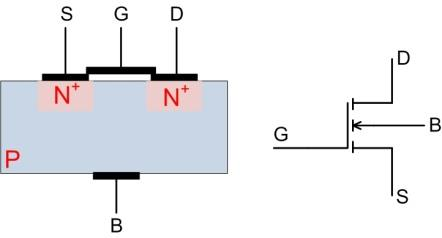
\includegraphics[width=0.7\linewidth]{Obrazky/ESOT/Otazka2/mosfetInduk}
		\caption{Indukovaný kanál.}
		\label{fig:indukMosfet}
	\end{subfigure}
	\begin{subfigure}[b]{0.48\textwidth}
		\centering
		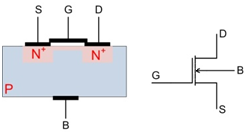
\includegraphics[width=0.7\linewidth]{Obrazky/ESOT/Otazka2/mosfetInteg}
		\caption{Integrovaný kanál.}
		\label{fig:integMosfet}
	\end{subfigure}	
\end{figure}
\begin{figure}[H]
	\centering
	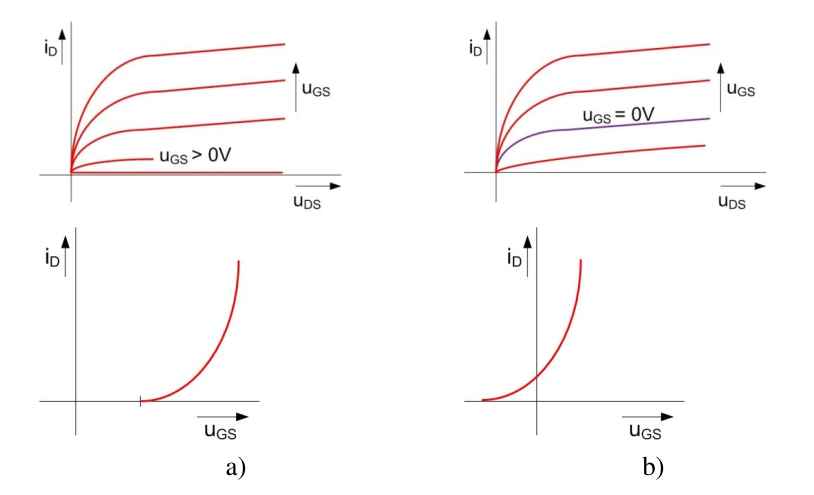
\includegraphics[width=0.7\linewidth]{Obrazky/ESOT/Otazka2/charInduk}
	\caption{Výstupná a prevodná charakteristika tranzistora IGFET s indukovaným kanálom (a) a trvalým kanálom (b)}
	\label{fig:charinduk}
\end{figure}
\begin{figure}[H]
	\centering
	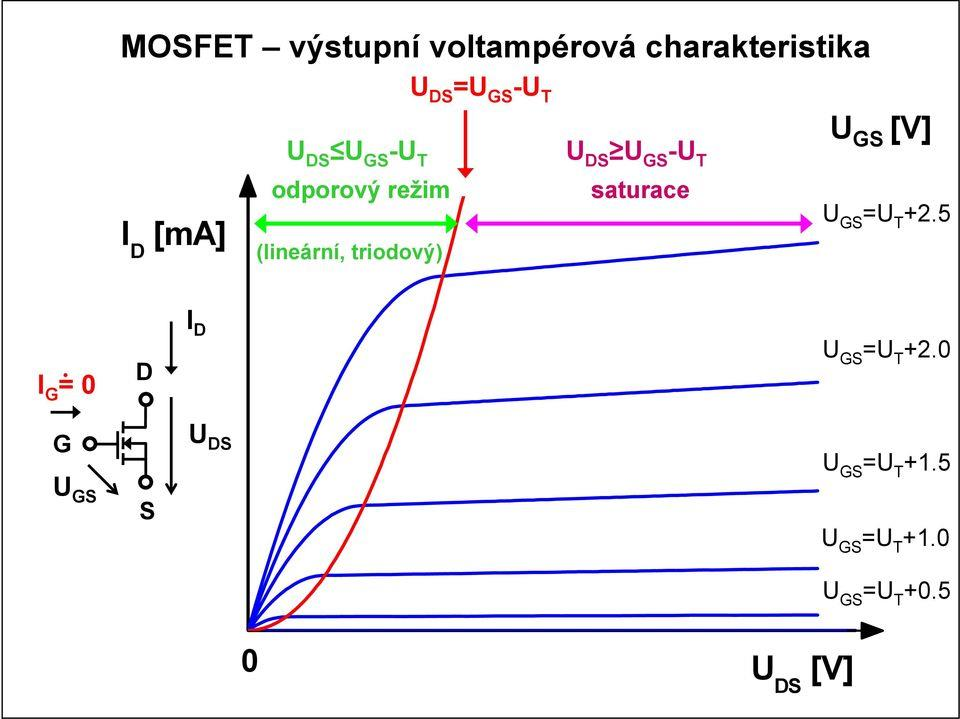
\includegraphics[width=0.7\linewidth]{Obrazky/ESOT/Otazka2/charMosfet}
	\caption{Výstupná voltampérová charakteristika MOSFET}
	\label{fig:charmosfet}
\end{figure}

\section{MESFET}
Tranzistor \textbf{MESFET} (Metal-Semiconductor FET) nahrádza prechod PN (JFET) alebo izolant (MOSFET) priamo prechodom kov-polovodič, ktorý vytvára tzv. \textbf{Schottkyho bariéru}. Používa sa predovšetkým pre vysokofrekvenčné a mikrovlnné aplikácie (často realizovaný na arsenide galitom – $\text{GaAs}$), kde absenciou izolačnej vrstvy alebo difúznych prechodov dosahuje extrémne vysoké rýchlosti a nízky šum, avšak vykazuje vyšší klidový prúd hradla pri nesprávnej polarizácii v porovnaní s MOSFET.
\begin{figure}[H]
	\centering
	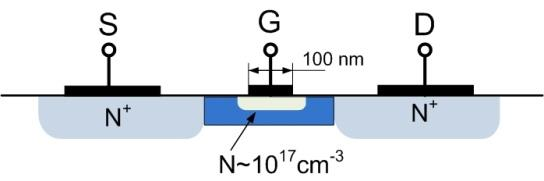
\includegraphics[width=0.7\linewidth]{Obrazky/ESOT/Otazka2/mesfetObrazok}
	\caption{Štruktúra tranzistora MESFET}
	\label{fig:mesfetobrazok}
\end{figure}
\section{Aplikácie a režimy činnosti tranzistorov FET}

Tranzistory FET (unipolárne tranzistory) môžu pracovať v rôznych režimoch v závislosti od požadovanej aplikácie. Podľa toho, v akom režime chceme tranzistor použiť, nastavujeme jeho pracovný bod:
\begin{itemize}
	\item \textbf{Tranzistor ako zdroj prúdu} – saturačný režim.
	\item \textbf{Tranzistor ako zosilňovač} – saturačný režim (pre dosiahnutie maximálnej strmosti).
	\item \textbf{Tranzistor ako spínač} – striedanie režimu odrezania (vypnutý) a triódového/saturačného režimu (zapnutý).
	\item \textbf{Tranzistor ako riadený odpor} – lineárny (aktívny) režim pri malých napätiach $U_{\text{DS}}$.
\end{itemize}

\section{FET ako prúdový zdroj (prúdové zrkadlá)}
V saturačnom režime vykazuje FET vlastnosti riadeného prúdového zdroja, kde je výstupný prúd nezávislý od napätia $U_{\text{DS}}$.

\begin{itemize}
	\item \textbf{Prúdová nora (Current Sink):} Prúdové zrkadlo realizované pomocou NMOS tranzistorov.
	\item \textbf{Prúdový zdroj (Current Source):} Prúdové zrkadlo realizované pomocou PMOS tranzistorov.
	\item \textbf{Pokročilé zapojenia prúdových zrkadiel:} Kaskódové prúdové zrkadlo, Wilsonovo prúdové zrkadlo, prúdové zrkadlo s regulovanou kaskádou.
\end{itemize}

\paragraph{Princíp zrkadlenia:}
Zapojenie sa nazýva zrkadlo, pretože vstupný prúd prvého tranzistora ($I_{\text{D1}}$) definuje riadiace napätie $U_{\text{GS}}$, ktoré sa prenáša na druhý tranzistor. Výstupný prúd ($I_{\text{D2}}$) je v presnom pomere so vstupným prúdom. Tento pomer je určený geometriou kanálov oboch MOSFETov, teda pomerom ich šírok ($W$) a dĺžok ($L$):
\begin{equation}
	\frac{I_{\text{D2}}}{I_{\text{D1}}} = \frac{\left(\frac{W_2}{L_2}\right)}{\left(\frac{W_1}{L_1}\right)}
\end{equation}

\paragraph{Vlastnosti prúdového zdroja s FET:}
\begin{itemize}
	\item Generujú konštantný prúd cez ľubovoľný rozsah napätia (rozsah je obmedzený podmienkou udržania tranzistora v saturácii).
	\item Výstupná impedancia je teoreticky nekonečne veľká (v reálnom MOS tranzistore je limitovaná dĺžkovou moduláciou kanála).
\end{itemize}

\paragraph{Podmienka činnosti:}
Riadiaci aj výstupný tranzistor ($M_1$ a $M_2$) musia byť bezpodmienečne udržiavané v \textbf{saturačnom režime}:
\begin{equation}
	U_{\text{DS}} \ge U_{\text{GS}} - U_{\text{P}}
\end{equation}

\begin{figure}[H]
	\centering
	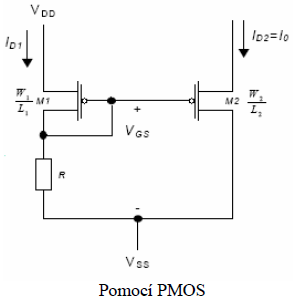
\includegraphics[width=0.35\linewidth]{Obrazky/ESOT/Otazka2/prudovyZdrojZrkadlo}
	\caption{Prúdové zrkadlo realizované pomocou PMOS.}
	\label{fig:prudovyzdrojzrkadlo}
\end{figure}


\section{FET ako zosilňovač}
Najčastejšie sa využíva unipolárny tranzistor v zapojení \textbf{SS} (so spoločným zdrojom – Source, analógia k zapojeniu SE s emitorom pri bipolárnych tranzistoroch).

\paragraph{Vlastnosti a podmienky:}
\begin{itemize}
	\item \textbf{Maximálna strmosť} prevodnej charakteristiky ($g_{\text{m}}$) sa dosahuje v \textbf{saturačnom režime}, preto je tento režim pre zosilňovače kľúčový.
	\item Pre zabezpečenie lineárnej činnosti v saturácii pri veľkých amplitúdach signálu je potrebné dostatočne \textbf{veľké napájacie napätie} $U_{\text{DD}}$.
	\item Nevýhodou oproti bipolárnym tranzistorom (BT) je \textbf{menšia strmosť} (typicky napr. $5\,\text{mS}$ pre FET oproti $50\,\text{mS}$ pre BT).
\end{itemize}

\paragraph{Nastavenie pracovného bodu:}
\begin{itemize}
	\item \textbf{Odporový delič v hradle} je nevyhnutný pre IGFET/MOSFET s indukovaným kanálom, pretože na ich otvorenie je potrebné kladné napätie ($U_{\text{P}} > 0$ pre NMOS).
	\item Pri JFEToch a IGFEToch s trvalým kanálom vykazuje pracovný bod menšiu závislosť od technologického rozptylu prahového napätia $U_{\text{P}}$.
	\item Úbytok napätia na rezistore $R_{\text{S}}$ v zapojení s automatickým predpätím nahrádza potrebu externého záporného zdroja pre dosiahnutie potrebného záporného napätia $U_{\text{GS}}$.
\end{itemize}
\begin{figure}[H]
	\centering
	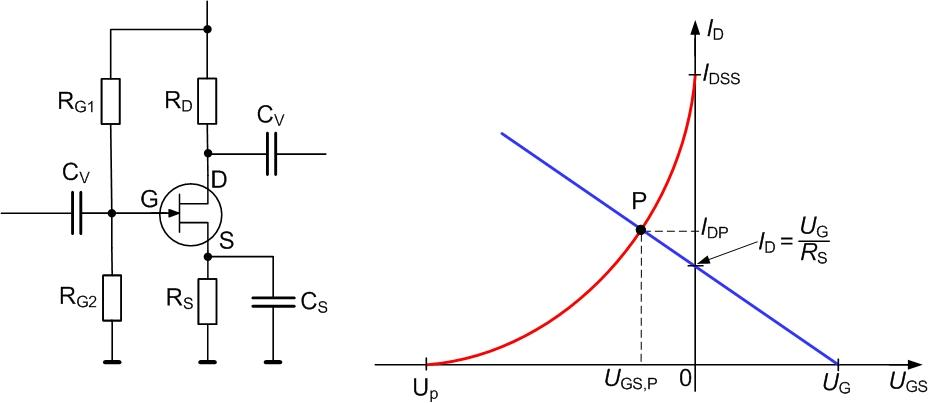
\includegraphics[width=0.7\linewidth]{Obrazky/ESOT/Otazka2/fetZosik}
	\caption{Zosilňovač JFET a nastavenie jeho pracovného bodu.}
	\label{fig:fetzosik}
\end{figure}

\section{FET ako spínač}
Využíva sa predovšetkým zapojenie so spoločným zdrojom (SS). Spínač pracuje v dvoch stavoch: bud je úplne zatvorený (režim odrezania), alebo plne otvorený (triódový režim s minimálnym úbytkom napätia).

\paragraph{Vlastnosti spínača s FET:}
\begin{itemize}
	\item \textbf{Absencia akumulácie náboja:} Keďže FET pracuje len s majoritnými nosičmi, nevzniká tu efekt akumulácie minoritných nosičov (známy z bipolárnych tranzistorov), čo umožňuje rýchle spínanie.
	\item \textbf{Doba zopnutia/rozopnutia} je primárne určená parazitnými kapacitami ($C_{\text{GS}} + C_{\text{GD}}$, resp. tzv. Millerovou kapacitou) a veľkosťou prúdu hradla $I_{\text{G}}$, ktorý tieto kapacity nabíja.
	\item Hoci je statický prúd hradla takmer nulový, na rýchle prenabitie kapacít pri spínaní je potrebný dynamický impulz prúdu hradla (typicky $I_{\text{G}} \approx 0,1\,\text{A} \div 1\,\text{A}$ počas trvania desiatok nanosekúnd, napr. $100\,\text{ns}$).
	\item Výhodou je veľmi \textbf{malý riadiaci príkon} v statickom stave.
\end{itemize}

\paragraph{Výkonové spínače (napr. MOSFET typu VDMOS):}
\begin{itemize}
	\item Pre $U_{\text{GS}} = 0\,\text{V}$ je spínač bezpečne rozopnutý, keďže prahové napätie býva $U_{\text{P}} \approx 4 \div 5\,\text{V}$.
	\item Dosahujú \textbf{veľké záverné napätia} ($1000 \div 1200\,\text{V}$).
\end{itemize}
	
	\section{FET ako riadený odpor (analógový spínač)}
	Ak tranzistor FET pracuje v \textbf{lineárnom (aktívnom) režime} pri veľmi malých napätiach $U_{\text{DS}}$ (blízko počiatku súradnicovej sústavy), kanál sa správa ako čistý odpor.
	
	\begin{itemize}
\item Využíva sa aktívna časť výstupnej charakteristiky, kde je sklon priamky (vodivosť kanála) priamo závislý od riadiaceho napätia $U_{\text{GS}}$.
\item \textbf{Dynamický odpor kanála} ($r_{\text{DS}}$) je možné plynule riadiť zmenou napätia $U_{\text{GS}}$. S rastúcim napätím $U_{\text{GS}}$ (nad prahovú hodnotu) odpor kanála klesá.
\end{itemize}
\begin{figure}[H]
	\centering
	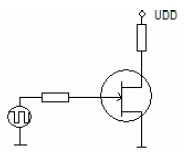
\includegraphics[width=0.15\linewidth]{Obrazky/ESOT/Otazka2/fetSpinac}
	\caption{Spínač s FET tranzistorom.}
	\label{fig:fetspinac}
\end{figure}

\section{Paralelná integrácia výkonových tranzistorov FET}
Výkonové parametre tranzistorov FET (najmä schopnosť viesť veľké prúdy a dosiahnuť extrémne malý odpor v zopnutom stave $R_{\text{DS(on)}}$) sa zvyšujú \textbf{rozširovaním kanála} (geometrický parameter šírky $W$, v texte označovaný ako $Z$), respektíve \textbf{paralelným radením} veľkého množstva čiastkových tranzistorových štruktúr (systémov) na jednom čipe.

\paragraph{Výhoda paralelného radenia pri FET:}
Na rozdiel od bipolárnych tranzistorov majú FETy kladný teplotný koeficient odporu kanála. Ak sa jeden z paralelných kanálov začne prehrievať, jeho odpor vzrastie, čím sa prúd prirodzene redistribuuje do ostatných, chladnejších kanálov. Vďaka tejto vlastnosti nedochádza k lokálnemu tepelnému zrúteniu (tzv. thermal runaway) a tranzistory FET sa dajú veľmi ľahko integrovať paralelne ako na úrovni čipu, tak aj ako diskrétne súčiastky v obvode.


\chapter{Tyristor, Triak, IGBT}
Jedná sa o viacvrstvové súčiastky. Ich princíp je založený na kombinácií PN prechodov a je podobný ako činnosť BJT.
\section{Tyristor}
\begin{itemize}
	\item Schopnosť spínať veľké prúdy, pri veľkom napätí.
	\item Označujú sa tak bistabilné polovodičové súčiastky s tromi a viacerými PN prechodmi.
%	\item Má schopnosť spínať obe polarity napätia.
	\item V podstate obsahuje dva BJT $\rightarrow$ PNP a NPN.
	\item Ľahko sa spína a udržuje v zopnutom stave.
	\subitem Kolektorový prúd každého tranzistora je bázovým prúdom protiľahlého tranzistora.
	\item Ťažšie sa vypína $\rightarrow$ prúd štruktúrou musí klesnúť pod určitú úroveň.
\end{itemize}
\begin{figure}[H]
	\centering
	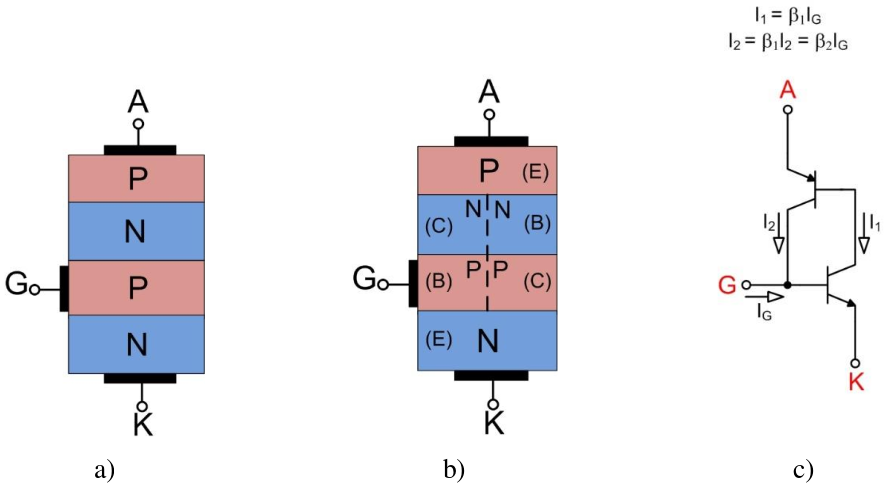
\includegraphics[width=0.7\linewidth]{Obrazky/ESOT/Otazka2/tyristorStruktura}
	\caption{Štruktúra tyristoru a jeho náhradná schéma.}
	\label{fig:tyristorstruktura}
\end{figure}
\section{Princíp činnosti tyristora}

Tyristor funguje ako riadený spínač realizovaný štvovrstvovou štruktúrou PNPN, ktorú si možno predstaviť ako zapojenie dvoch komplementárnych bipolárnych tranzistorov (PNP a NPN) spojených v uzavretej slučke s kladnou spätnou väzbou.

\paragraph{Základné stavy súčiastky:}
\begin{itemize}
	\item \textbf{Záverný stav ($U_{\text{AK}} < 0$):} Krajné prechody štruktúry sú polarizované v závernom smere. Kladná spätná väzba sa nemôže uzavrieť, tyristorom tečie len minimálny záverný prúd a súčiastka je nepriechodná.
	\item \textbf{Blokujúci stav ($U_{\text{AK}} > 0, I_{\text{G}} = 0$):} Krajné prechody sú v priepustnom smere, avšak stredný spoločný prechod (báza-kolektor) je polarizovaný v závernom smere. Blokuje prechod prúdu, pričom prúdové zosilňovacie činitele oboch fiktívnych tranzistorov sú pri malých prúdoch príliš nízke na to, aby sa spustila lavínová reakcia. Tyristor zostáva rozopnutý.
	\item \textbf{Zopnutý stav ($U_{\text{AK}} > 0, I_{\text{G}} > 0$):} Ak do riadiacej elektródy (hradla) vnútime prúdový impulz $I_{\text{G}}$, začne tiecť prúd bázou tranzistora NPN. Tento prúd sa zosilní a stane sa bázovým prúdom tranzistora PNP. Ten ho opätovne zosilní a dodá späť do bázy NPN. Vzniká \textbf{silná kladná spätná väzba}. Prúdy oboch tranzistorov sa navzájom lavínovito umocňujú, až kým stredný blokujúci prechod neprejde do saturácie. Tyristor sa úplne otvorí (zopne) a napäťový úbytok na ňom klesne na minimum.
\end{itemize}
\begin{figure}[H]
	\centering
	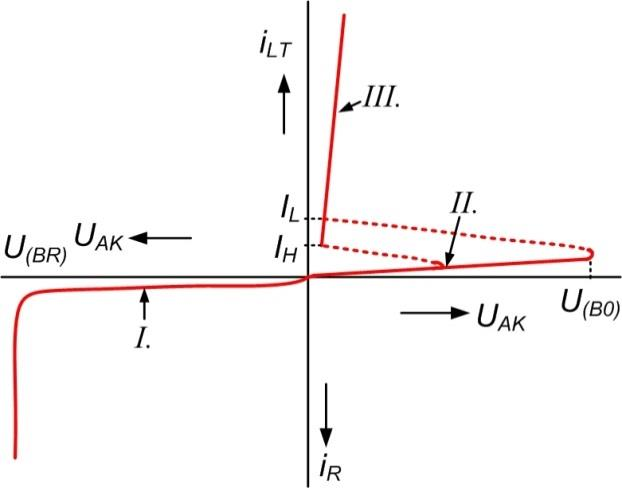
\includegraphics[width=0.35\linewidth]{Obrazky/ESOT/Otazka2/vystupnaTyristor}
	\caption{Výstupná charakteristika zpätne záverného tyristora.}
	\label{fig:vystupnatyristor}
\end{figure}

\paragraph{Udržanie zopnutého stavu a vypnutie:}
Po zopnutí preberá vnútorná kladná spätná väzba plnú kontrolu nad štruktúrou. Tyristor preto \textbf{zostáva zopnutý aj po odpojení riadiaceho prúdu $I_{\text{G}}$}. Na jeho opätovné vypnutie (prechod do blokujúceho stavu) je nutné externým obvodom znížiť pretekajúci prúd anódy $I_{\text{A}}$ pod kritickú hodnotu, tzv. \textbf{prúdudržiavací prúd} $I_{\text{H}}$ (Holding current), alebo zmeniť polaritu napätia $U_{\text{AK}}$.

\section{Triak}

Triak (\textit{Triode AC Switch}) je päťvrstvová polovodičová štruktúra určená na obojsmerné riadenie striedavého prúdu. Na rozdiel od klasického tyristora dokáže spínať prúd v oboch smeroch.
\paragraph{Štruktúra triaku:}
Základnú štruktúru si možno predstaviť ako dva tyristory zapojené antiparalelne (proti sebe) na jednom čipe. 
\begin{itemize}
	\item Pozostáva z vrstiev striedajúcich sa typov vodivosti, pričom hlavné elektródy sa označujú ako \textbf{A1} (anóda 1) a \textbf{A2} (anóda 2). Diódové prechody polarizované v závernom smere sú potlačené tým, že sú skratované kontaktmi týchto hlavných elektród.
	\item Praktická štruktúra je doplnená o \textbf{pomocnú oblasť $N_{\text{G}}$} v blízkosti riadiacej elektródy \textbf{G} (hradla). Táto modifikácia umožňuje galvanické spojenie riadiacich obvodov s elektródou A1 a zabezpečuje spúšťanie triaku kladným aj záporným prúdom hradla ($\pm I_{\text{G}}$) pri oboch polaritách napätia medzi hlavnými elektródami.
\end{itemize}
\begin{figure}[H]
	\centering
	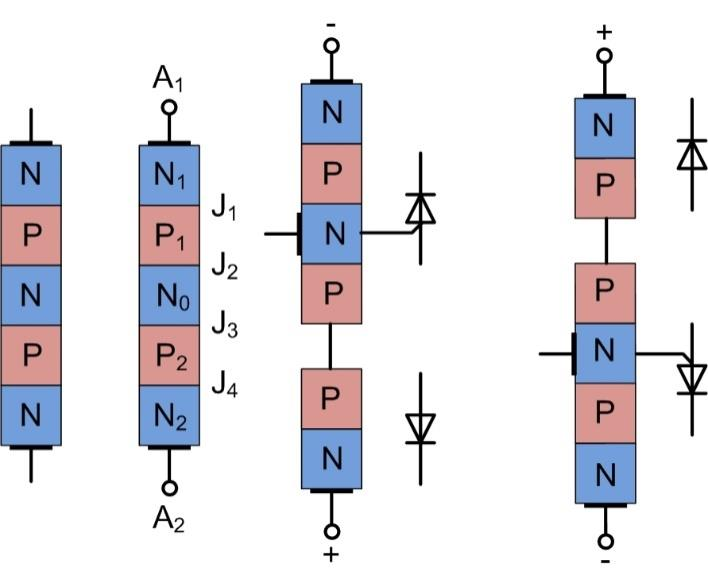
\includegraphics[width=0.35\linewidth]{Obrazky/ESOT/Otazka2/triakStruktura}
	\caption{Štruktúra triaku.}
	\label{fig:triakstruktura}
\end{figure}
\begin{figure}[H]
	\centering
	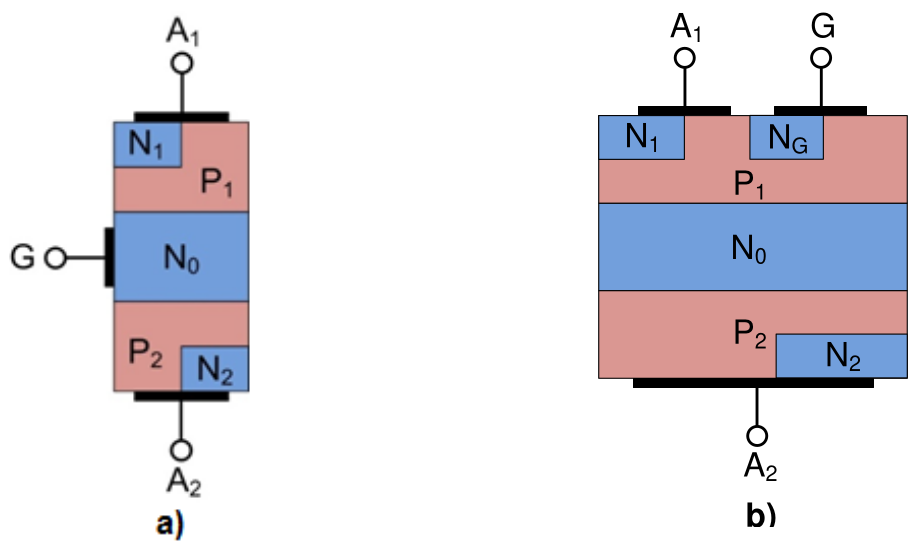
\includegraphics[width=0.5\linewidth]{Obrazky/ESOT/Otazka2/strukturaTriak}
	\caption{Štruktúra triaku symetrická (a), a s pomocnou oblasťou $N_G$ (b).}
	\label{fig:strukturatriak}
\end{figure}

\paragraph{Princíp činnosti pri polarite A2 kladnej proti A1:}
V tomto stave je prechod $P_2N_2$ v závernom smere a skratovaný kontaktom A2, takže je nefunkčný. Spúšťanie prebieha nasledovne:
\begin{itemize}
	\item \textbf{Pri kladnom impulze ($+I_{\text{G}}$):} Spustí sa priamo hlavný tyristor štruktúry $P_2N_0P_1N_1$ z elektródy G cez oblasť $P_1$ (tzv. \textit{riadenie do blízkej bázy}).
	\item \textbf{Pri zápornom impulze ($-I_{\text{G}}$):} Najprv sa zopne vedľajší pomocný tyristor $P_2N_0P_1N_{\text{G}}$ (z elektródy A1 cez oblasť $P_1$). Jeho následné presýtenie nosičmi okamžite vyvolá zopnutie hlavného tyristora.
\end{itemize}

\paragraph{Princíp činnosti pri polarite A2 zápornej proti A1:}
Pri tejto polarite prebieha mechanizmus cez proces označovaný ako \textit{riadenie do vzdialenej bázy} (oblasť $N_0$):
\begin{enumerate}
	
\item  Zásadnú úlohu tu zohráva pomocný tranzistor $N_{\text{G}}P_1N_1$, ktorý sa uvedie do zopnutého stavu pri oboch polaritách riadiaceho prúdu ($\pm I_{\text{G}}$).
\item  Po zopnutí tohto tranzistora sa jeho báza v oblasti $P_1$ zaplní minoritnými nosičmi (elektrónmi). Keď ich koncentrácia dostatočne stúpne, začnú tieto nosiče prenikať (difundovať) cez prechod do vzdialenejšej oblasti $N_0$.
\item  Elektróny preniknuté do oblasti $N_0$ tu narušia nábojovú neutralitu, čím v oblasti $N_0$ vznikne záporný potenciál a začne sa otvárať prechod $P_1N_0$.
\item  Následkom tohto záporného potenciálu začnú z oblasti $P_1$ do oblasti $N_0$ plynúť diery. Tým sa pootvorí vnútorný tranzistor $P_2N_0P_1$.
\item  Keďže tranzistor $P_2N_0P_1$ je súčasťou komplementárnej štruktúry tyristora $N_2P_2N_0P_1$, jeho otvorenie vyvolá regeneratívny proces (kladnú spätnú väzbu) a zopne sa celá hlavná štruktúra triaku v opačnom smere.
\end{enumerate}
\begin{figure}[H]
	\centering
	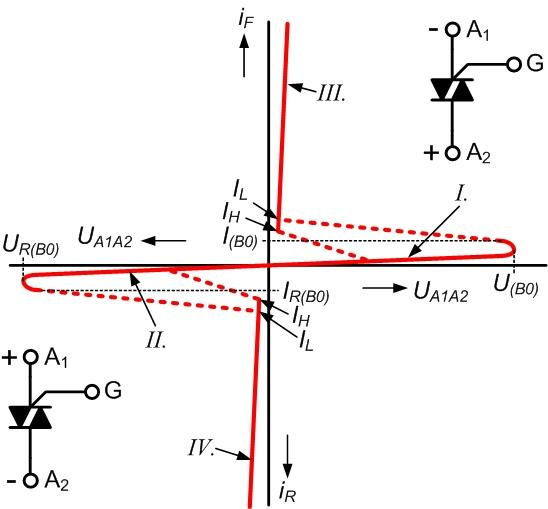
\includegraphics[width=0.35\linewidth]{Obrazky/ESOT/Otazka2/vystupnaTriak}
	\caption{Výstupná charakteristika Triaku.}
	\label{fig:vystupnatriak}
\end{figure}

\section{IGBT}
IGBT vznikol zo štruktúry VDMOS, pričom bol nahradený substrát N+ substrátom P+.
IGBT: Insulated Gate Bipolar Transistor.
\section{Princíp činnosti a vlastnosti IGBT}

Tento mechanizmus popisuje činnosť bipolárneho tranzistora s izolovaným hradlom (\textbf{IGBT}), ktorý kombinuje výhody riadenia napätím (vlastnosť MOSFETu) a nízkych strát v zopnutom stave (vlastnosť bipolárneho tranzistora).

\paragraph{Princíp činnosti a modulácia conductivity:}
\begin{itemize}
	\item \textbf{Vznik kanála a injekcia nosičov:} Po priložení kladného napätia na riadiacu elektródu (hradlo) sa pod ňou vytvorí \textbf{inverzná vrstva} (kanál typu N). Tento kanál vodivo prepojí emitorovú oblasť $\text{N}^+$ s vnútornou oblasťou bázy $\text{N}$. Vplyvom tohto prepojenia a polarity priloženého hlavného napätia sa začne otvárať spodný prechod $\text{P}^+\text{N}$, čo vyvolá masívnu \textbf{injekciu minoritných nosičov (dier)} zo substrátu $\text{P}^+$ do slabo dotovanej oblasti bázy $\text{N}$.
	\item \textbf{Modulácia vodivosti:} Táto injekcia dier výrazne zaplaví oblasť bázy nábojom, čím dramaticky \textbf{znižuje sériový odpor} celej štruktúry MOS (jav sa nazýva modulácia vodivosti). To umožňuje dosiahnuť extrémne vysoké prúdové hustoty pri zachovaní relatívne malého odporu zopnutého tranzistora.
\end{itemize}

\paragraph{Oblasti nasadenia a obmedzenia:}
\begin{itemize}
	\item \textbf{Vhodné aplikácie:} Vďaka tejto štruktúre sú IGBT tranzistory ideálne pre výkonové aplikácie vyžadujúce \textbf{vysoké blokovacie napätia} (stovky až tisíce voltov) a súčasne \textbf{veľké pretekajúce prúdy} (napr. frekvenčné meniče, pohony, trakčné vedenia).
	\item \textbf{Nevýhoda napäťového úbytku:} Keďže je v hlavnom prúdovom chodníku sériovo zapojený PN prechod (spomínaná diódová časť $\text{P}^+\text{N}$), súčiastka vykazuje pomerne \textbf{veľký prahový napäťový úbytok} (typicky $0,7\,\text{V}$ až $1,5\,\text{V}$) aj pri minimálnych prúdoch. Z tohto dôvodu je IGBT úplne nevhodný pre nízkonapäťové aplikácie, kde sa vyžaduje úbytok menší ako $0,7\,\text{V}$ – v takých prípadoch ho jednoznačne prekonáva klasický výkonový MOSFET.
\end{itemize}
\begin{figure}[H]
	\centering
	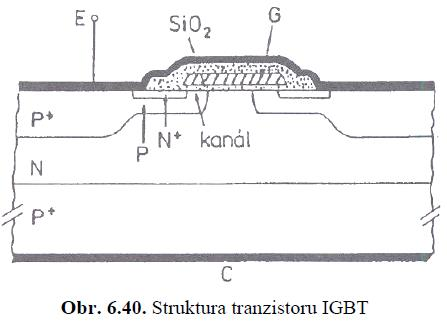
\includegraphics[width=0.35\linewidth]{Obrazky/ESOT/Otazka2/IGBT}
	\caption{Štruktúra IGBT tranzistora.}
	\label{fig:igbt}
\end{figure}
\begin{figure}[H]
	\centering
	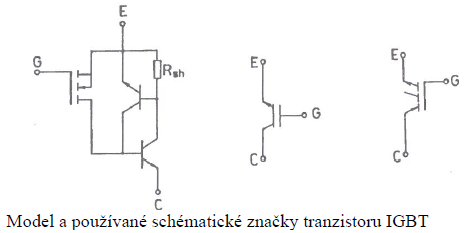
\includegraphics[width=0.35\linewidth]{Obrazky/ESOT/Otazka2/IGBTnahradnyObvod}
	\caption{Náhradný obvod IGBT.}
	\label{fig:igbtnahradnyobvod}
\end{figure}


\section{Fázové riadenie tyristora}

Fázové riadenie je základný spôsob regulácie striedavého výkonu dodávaného do záťaže. Využíva prirodzenú vlastnosť tyristorov a triakov – \textbf{samočinné vypnutie}, keď pretekajúci prúd v striedavom obvode klesne na nulu (na konci každej polvlny). Aby súčiastka v ďalšej polvlne opäť viedla prúd, musí byť znova zapálená riadiacim impulzom.

\paragraph{Princíp fázovej regulácie:}
Výkon odovzdávaný do záťaže sa reguluje \textbf{časovým oneskorením spúšťacieho impulzu $I_{\text{G}}$} oproti okamihu, kedy napájacie napätie prechádza nulou. 

\begin{itemize}
	\item \textbf{Maximálny výkon (Minimálne oneskorenie):} Impulz prichádza ihneď po prechode napätia nulou ($\alpha \approx 0^{\circ}$). Tyristor je otvorený takmer počas celej polvlny a do záťaže tečie maximálny prúd.
	\item \textbf{Minimálny výkon (Maximálne oneskorenie):} Impulz je posunutý až na samotný koniec polvlny ($\alpha \approx 180^{\circ}$). Tyristor sa otvorí len na veľmi krátky čas (alebo vôbec), takže výkon v záťaži je minimálny alebo nulový.
\end{itemize}
\begin{figure}[H]
	\centering
	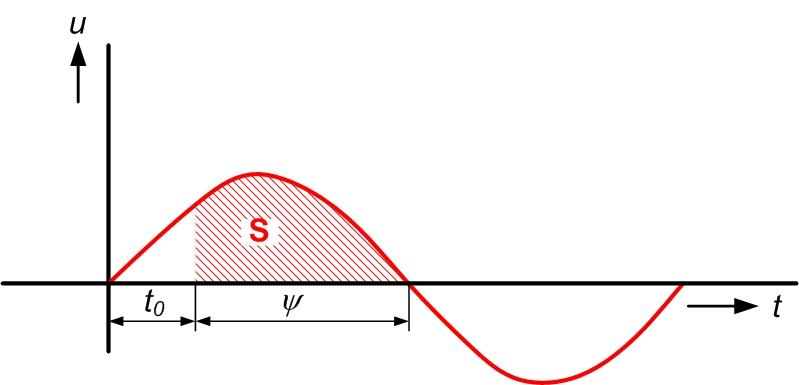
\includegraphics[width=0.4\linewidth]{Obrazky/ESOT/Otazka2/fazoveRiadenie}
	\caption{Princíp fázového riadenia v obvodoch striedavého prúdu.}
	\label{fig:fazoveriadenie}
\end{figure}

\section{Typy zapojenia pre celovlnnú reguláciu}

Keďže klasický tyristor vedie prúd iba v jednom smere (počas kladnej polvlny $U_{\text{AK}} > 0$), pre plnohodnotnú celovlnnú reguláciu v obvodoch striedavého prúdu sa využívajú tri hlavné konštrukčné prístupy:

\subsubsection{1. Antiparalelné zapojenie dvoch tyristorov}
Dva tyristory sú zapojené paralelne, ale s opačnou polaritou (proti sebe). Každý tyristor spracováva jednu polvlnu striedavého napätia.
\begin{itemize}
	\item \textbf{Vlastnosti:} Bežne sa používa pre \textbf{vysoké výkony nad $10\,\text{kW}$}.
	\item \textbf{Úskalia:} Riadiace obvody musia zabezpečiť absolútne presný súbeh časovania oboch impulzov (najmä pri induktívnej záťaži). Riadiace obvody musia byť \textbf{galvanicky oddelené} a špičkovo izolované, keďže rozdiel potenciálov medzi katódami tyristorov môže v aplikáciách vysokého napätia presiahnuť aj $10\,\text{kV}$.
\end{itemize}
\begin{figure}[H]
	\centering
	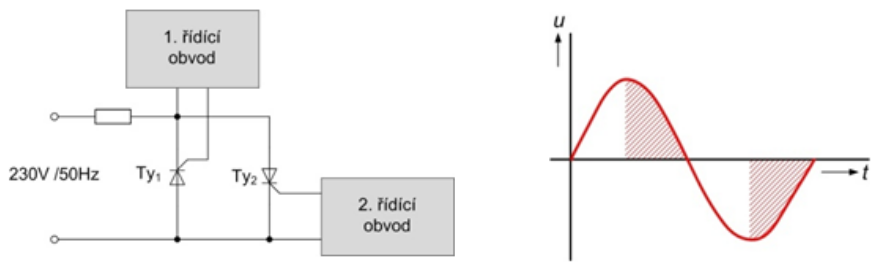
\includegraphics[width=0.7\linewidth]{Obrazky/ESOT/Otazka2/fazoveRiadenie3}
	\caption{Celovlnná regulácia pri antiparalelnom napätí.}
	\label{fig:fazoveriadenie3}
\end{figure}

%\subsubsection{2. Zapojenie s jedným triakom}
%Triak nahradzuje obidva antiparalelné tyristory, pretože je sám o sebe schopný viesť prúd v oboch smeroch a spúšťať sa impulzmi ľubovoľnej polarity.
%\begin{itemize}
%	\item \textbf{Vlastnosti:} Konštrukčne najjednoduchšie a ekonomické zapojenie. Vhodné pre \textbf{stredné výkony do cca $10\,\text{kW}$} (napr. domáce stmievače, regulácia otáčok ručného náradia).
%	\item \textbf{Úskalia:} Pri induktívnej záťaži sa môžu vyskytnúť problémy so spoľahlivosťou zatvárania (komutáciou) kvôli fázovému posunu medzi prúdom a napätím.
%\end{itemize}

\subsubsection{3. Zapojenie tyristorov s usmerňovacím mostíkom}
Tyristory sú umiestnené vo vnútri jednosmernej diagonály diódového usmerňovacieho mostíka.
\begin{itemize}
	\item \textbf{Výhoda:} Obidva tyristory môžu byť riadené z \textbf{jedného spoločného zdroja riadiacich impulzov}. Tým sa úplne eliminuje riziko nesymetrického posunu spúšťania medzi kladnou a zápornou polvlnou.
	\item \textbf{Nevýhoda:} Podstatne \textbf{vyššia výkonová strata}. Prúd prechádza vždy nielen cez tyristor, ale aj cez diódy mostíka, na ktorých vzniká dodatočný napäťový úbytok a s ním spojené teplo.
\end{itemize}
\begin{figure}
	\centering
	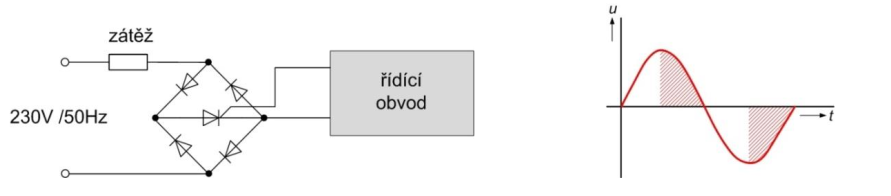
\includegraphics[width=0.7\linewidth]{Obrazky/ESOT/Otazka2/fazoveRiadenie4}
	\caption{Celovlnná regulácia s usmerňovačom.}
	\label{fig:fazoveriadenie4}
\end{figure}

%\section{Pracovné režimy tyristora}
%
%Podľa polarity priloženého napätia $U_{\text{AK}}$ môže tyristor pracovať v dvoch základných režimoch:
%
%\begin{enumerate}
%	\item \textbf{Záverný režim ($U_{\text{AK}} < 0$):} Na anode je záporné napätie. Krajné prechody (emitor-báza oboch fiktívnych tranzistorov) sú polarizované v závernom smere a nesú celé priložené napätie, zatiaľ čo spoločný stredný prechod (báza-kolektor) je v propustnom smere. Štruktúra sa správa ako dve diódy zapojené v sérii v závernom smere. Kladná spätná väzba sa nemôže uzavrieť, takže zopnutie nenastane.
%	
%	\item \textbf{Blokujúci režim ($U_{\text{AK}} > 0$):} Na anode je kladné napätie. Krajné prechody sú polarizované v priepustnom smere, spoločný stredný prechod je v závernom smere. Tranzistory si môžu navzájom odovzdávať prúd, čím vzniká riziko uzavretia kladnej spätnej väzby a zopnutia štruktúry.
%\end{enumerate}
%
%\paragraph{Spôsoby zopnutia tyristora v blokujúcom režime:}
%\begin{itemize}
%	\item \textbf{Prúdom hradla $I_{\text{G}}$ (žiaduce):} Riadiaci impulz je zosilnený kladnou spätnou väzbou a štruktúra rýchlo zopne. K uzavretiu spätnej väzby dôjde až po dosiahnutí kritickej veľkosti prúdu $I_{\text{G}}$.
%	\item \textbf{Prekročením napätia $U_{\text{AKBR}}$ (nežiaduce):} Pri kritickom zvýšení napätia rastie záverný prúd stredného prechodu lavínovým násobením ($I_{\text{CB0}}$). Po prekročení kritickej hodnoty prúdu tyristor zopne.
%	\item \textbf{Zvýšením teploty (nežiaduce):} S rastúcou teplotou generácie nosičov stúpa záverný prúd stredného prechodu, čo vyvolá rovnaký mechanizmus samovoľného zopnutia.
%	\item \textbf{Strmosťou nárastu napätia $d U_{\text{AK}} / d t$ (nežiaduce):} Bariérová kapacita stredného prechodu $C_{\text{BC}}$ prepustí pri rýchlej zmene napätia prúdový impulz ($i = C_{\text{BC}} \cdot \frac{dU_{\text{AK}}}{dt}$), ktorý otvorí emitorové prechody rovnako ako externý prúd hradla.
%\end{itemize}
%
%\section{Štruktúra s deleným emitorom}
%Na potlačenie nežiaducich spôsobov zopnutia (teplotou, strmosťou či napätím) sa využíva \textbf{konštrukcia s deleným emitorom}, kde je oblasť emitora tranzistora NPN rozdelená a čiastočne skratovaná priamo kontaktom katódy.
%
%\begin{itemize}
%	\item \textbf{Blokovanie:} Záverný prúd stredného prechodu tečie z bázy tranzistora NPN priamo do kontaktu katódy. Obchádza tak priepustný prechod báza-emitor a bráni nežiaducemu zopnutiu.
%	\item \textbf{Riadené zopnutie:} Ak do hradla vnútime dostatočne veľký prúd $I_{\text{G}}$, úbytok napätia na odporovom materiáli bázy narastie natoľko, že sa prechod báza-emitor predsa len otvorí, vnúti prúd susednému tranzistoru PNP a tyristor cielene zopne. Nevýhodou tejto odolnejšej štruktúry je potreba podstatne väčšieho spúšťacieho prúdu $I_{\text{G}}$.
%\end{itemize}






